\chapter{Ойындар теориясы}

Бұл тарауда кездейсоқ элементтерді қамтымайтын, екі ойыншы 
ойнайтын ойындарды қарастыратын боламыз. Біздің мақсатымыз --
қарсыласымыз қандай да бір жүріс жасағанда әрдайым жеңіске 
жетуді қамтамасыз ететін стратегияны 
табу немесе ондай стратегия жоқ екенін хабарлау. % (егер ондай стратегия бар болса). 

% In this chapter, we will focus on two-player
% games that do not contain random elements.
% Our goal is to find a strategy that we can
% follow to win the game
% no matter what the opponent does,
% if such a strategy exists.

Мұндай ойындарға арналған жалпы стратегия бар екені белгілі болып отыр
және ойындарды \key{ним теориясы} арқылы талдауымызға болады.
Алдымен ойыншылар таяқтар үйіндісінен таяқтарды алып отыратын ойынды
талдаймыз, содан кейін стратегияны басқа ойындарға
жалпылайтын боламыз. 

% It turns out that there is a general strategy
% for such games,
% and we can analyze the games using the \key{nim theory}.
% First, we will analyze simple games where
% players remove sticks from heaps,
% and after this, we will generalize the strategy
% used in those games to other games.

\section{Ойын күйлері}

Басында $n$ таяқтардан тұратын үйінді берілген 
ойынды қарастырайық. $A$ және $B$ ойыншылары кезек бойынша
жүреді және $A$ ойыншысы бірінші бастайды. Әр жүрісте
ойыншы үйіндіден 1, 2 немесе 3 таяқ алу қажет. Ең соңғы таяқты алған ойыншы ойынды жеңеді. 

% Let us consider a game where there is initially
% a heap of $n$ sticks.
% Players $A$ and $B$ move alternately,
% and player $A$ begins.
% On each move, the player has to remove
% 1, 2 or 3 sticks from the heap,
% and the player who removes the last stick wins the game.

Мысалы, егер $n=10$ болса, ойын келесідей жалғаса алады:
% For example, if $n=10$, the game may proceed as follows:
\begin{itemize}[noitemsep]
\item $A$ ойыншысы 2 таяқты алады (8 таяқ қалды).
\item $B$ ойыншысы 3 таяқты алады (5 таяқ қалды).
\item $A$ ойыншысы 1 таяқты алады (4 таяқ қалды).
\item $B$ ойыншысы 2 таяқты алады (2 таяқ қалды).
\item $A$ ойыншысы 2 таяқты алады және ойынды жеңеді.
\end{itemize}

Ойын $0,1,2,\ldots,n$ күйлерден тұрады, ол 
қалған таяқтар санына сәйкес келеді. 

% This game consists of states $0,1,2,\ldots,n$,
% where the number of the state corresponds to
% the number of sticks left.

\subsubsection{Ұтыс және ұтылыс күйлері}

\index{ұтыс күйі}
\index{ұтылыс күйі}

\key{Ұтыс күйі} -- егер ойыншы оңтайлы түрде ойнайтын болса,
әрдайым ұтатын күй. Ал \key{ұтылыс күйі} -- егер қарсыласы 
оңтайлы түрде ойнайтын болса, әрдайым ұтылатын күй. 
Ойынның әр күйін ұтыс немесе ұтылыс күйлеріне топтастырсақ болады.

% A \key{winning state} is a state where
% the player will win the game if they
% play optimally,
% and a \key{losing state} is a state
% where the player will lose the game if the
% opponent plays optimally.
% It turns out that we can classify all states
% of a game so that each state is either
% a winning state or a losing state.

Жоғарыдағы ойында 0 күйі -- анық ұтылыс күйі. Өйткені ойыншы ешқандай
жүріс жасай алмайды. 1, 2 және 3 күйлері -- ұтыс күйлер. Өйткені
1, 2 немесе 3 таяқты алсақ, ойынды ұтатын боламыз. 
4 күйі -- ұтылыс күй, себебі кез келген жүріс
қарсылас үшін ұтыс күйге жетелейді.

% In the above game, state 0 is clearly a
% losing state, because the player cannot make
% any moves.
% States 1, 2 and 3 are winning states,
% because we can remove 1, 2 or 3 sticks
% and win the game.
% State 4, in turn, is a losing state,
% because any move leads to a state that
% is a winning state for the opponent.

Жалпы айтқанда егер қазіргі күйден ұтылыс күйіне апаратын
жүріс болса, онда қазіргі күй ұтыс күйі болады. Әйтпесе қазіргі 
күй ұтылыс күйі болады. Осы бақылауды қолдана отыра ойынның 
барлық күйлерін топтастыруға болады. 

% More generally, if there is a move that leads
% from the current state to a losing state,
% the current state is a winning state,
% and otherwise the current state is a losing state.
% Using this observation, we can classify all states
% of a game starting with losing states where
% there are no possible moves.

Жоғарыдағы ойынның $0 \ldots 15$ күйлері келесі ретпен топтастырылады
($W$ ұтыс күйін белгілейді және $L$ ұтылыс күйін белгілейді):

% The states $0 \ldots 15$ of the above game
% can be classified as follows
% ($W$ denotes a winning state and $L$ denotes a losing state):
\begin{center}
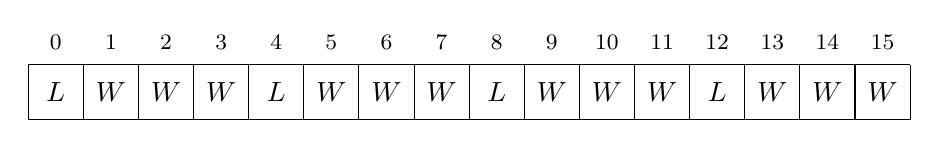
\begin{tikzpicture}[scale=0.7]
\draw (0,0) grid (16,1);

\node at (0.5,0.5) {$L$};
\node at (1.5,0.5) {$W$};
\node at (2.5,0.5) {$W$};
\node at (3.5,0.5) {$W$};
\node at (4.5,0.5) {$L$};
\node at (5.5,0.5) {$W$};
\node at (6.5,0.5) {$W$};
\node at (7.5,0.5) {$W$};
\node at (8.5,0.5) {$L$};
\node at (9.5,0.5) {$W$};
\node at (10.5,0.5) {$W$};
\node at (11.5,0.5) {$W$};
\node at (12.5,0.5) {$L$};
\node at (13.5,0.5) {$W$};
\node at (14.5,0.5) {$W$};
\node at (15.5,0.5) {$W$};

\footnotesize
\node at (0.5,1.4) {$0$};
\node at (1.5,1.4) {$1$};
\node at (2.5,1.4) {$2$};
\node at (3.5,1.4) {$3$};
\node at (4.5,1.4) {$4$};
\node at (5.5,1.4) {$5$};
\node at (6.5,1.4) {$6$};
\node at (7.5,1.4) {$7$};
\node at (8.5,1.4) {$8$};
\node at (9.5,1.4) {$9$};
\node at (10.5,1.4) {$10$};
\node at (11.5,1.4) {$11$};
\node at (12.5,1.4) {$12$};
\node at (13.5,1.4) {$13$};
\node at (14.5,1.4) {$14$};
\node at (15.5,1.4) {$15$};
\end{tikzpicture}
\end{center}

Бұл ойынды оңай түрде талдауға болады:
егер $k$ 4-ке бөлінсе, $k$ күйі ұтылыс күйі болады, басқа жағдайда, ол ұтыс күйі болмақ. Бұл ойынды ұтудың
оңай жолы -- әрдайым таяқтардың саны 4-ке 
бөлінетін күйге апаратын жүріс жасау. Ақырында
таяқтар қалмайды және қарсылас жеңіледі. 

% It is easy to analyze this game:
% a state $k$ is a losing state if $k$ is
% divisible by 4, and otherwise it
% is a winning state.
% An optimal way to play the game is
% to always choose a move after which
% the number of sticks in the heap
% is divisible by 4.
% Finally, there are no sticks left and
% the opponent has lost.

Бұл стратегия әрине біздің жүрісіміздегі 
таяқтар санының 4-ке \emph{бөлінбеуін} талап
етеді. Егер бөлінсе, біз ештеңе істей алмаймыз. Егер қарсыласымыз оңтайлы ойнайтын болса, әрдайым жеңеді. 

% Of course, this strategy requires that
% the number of sticks is \emph{not} divisible by 4
% when it is our move.
% If it is, there is nothing we can do,
% and the opponent will win the game if
% they play optimally.

\subsubsection{Күйлер графы}

Енді басқа таяқтар ойынын қарастырайық. Бұл
ойынның шартына сәйкес әр $k$ күйде $k$-дан кіші және $k$ $x$-ке бөлінуі тиіс кез келген таяқтарды алуымызға болады. Мысалы 8 күйінде 
1, 2 немесе 4 таяқтарды алсақ болады, бірақ 7 күйінде тек
1 таяқты алуға болады. 

% Let us now consider another stick game,
% where in each state $k$, it is allowed to remove
% any number $x$ of sticks such that $x$
% is smaller than $k$ and divides $k$.
% For example, in state 8 we may remove
% 1, 2 or 4 sticks, but in state 7 the only
% allowed move is to remove 1 stick.

Келесі сурет ойынның $1 \ldots 9$ күйлерін 
төбелері күй болатын және қырлары жүріс болатын
\key{күйлер графы} ретінде көрсетеді:

% The following picture shows the states
% $1 \ldots 9$ of the game as a \key{state graph},
% whose nodes are the states and edges are the moves between them:

\begin{center}
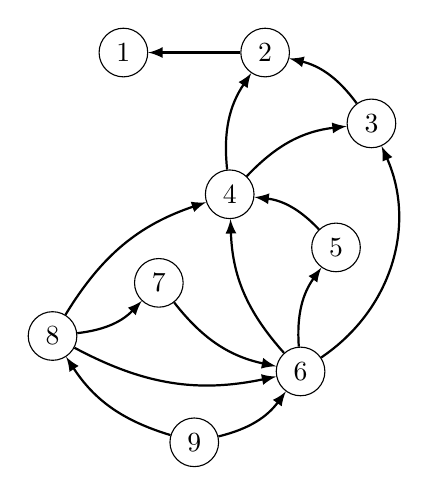
\begin{tikzpicture}[scale=0.9]
\node[draw, circle] (1) at (0,0) {$1$};
\node[draw, circle] (2) at (2,0) {$2$};
\node[draw, circle] (3) at (3.5,-1) {$3$};
\node[draw, circle] (4) at (1.5,-2) {$4$};
\node[draw, circle] (5) at (3,-2.75) {$5$};
\node[draw, circle] (6) at (2.5,-4.5) {$6$};
\node[draw, circle] (7) at (0.5,-3.25) {$7$};
\node[draw, circle] (8) at (-1,-4) {$8$};
\node[draw, circle] (9) at (1,-5.5) {$9$};

\path[draw,thick,->,>=latex] (2) -- (1);
\path[draw,thick,->,>=latex] (3) edge [bend right=20] (2);
\path[draw,thick,->,>=latex] (4) edge [bend left=20] (2);
\path[draw,thick,->,>=latex] (4) edge [bend left=20] (3);
\path[draw,thick,->,>=latex] (5) edge [bend right=20] (4);
\path[draw,thick,->,>=latex] (6) edge [bend left=20] (5);
\path[draw,thick,->,>=latex] (6) edge [bend left=20] (4);
\path[draw,thick,->,>=latex] (6) edge [bend right=40] (3);
\path[draw,thick,->,>=latex] (7) edge [bend right=20] (6);
\path[draw,thick,->,>=latex] (8) edge [bend right=20] (7);
\path[draw,thick,->,>=latex] (8) edge [bend right=20] (6);
\path[draw,thick,->,>=latex] (8) edge [bend left=20] (4);
\path[draw,thick,->,>=latex] (9) edge [bend left=20] (8);
\path[draw,thick,->,>=latex] (9) edge [bend right=20] (6);
\end{tikzpicture}
\end{center}

Ойынның ақырғы күйі әрдайым 1, және ол ұтылыс күйі, себебі
біз ешқандай жарамды жүріс жасай алмаймыз. 
$1 \ldots 9$ күйлері төмендегідей топтастырылады:

% The final state in this game is always state 1,
% which is a losing state, because there are no
% valid moves.
% The classification of states $1 \ldots 9$
% is as follows:

\begin{center}
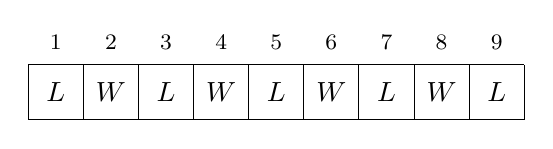
\begin{tikzpicture}[scale=0.7]
\draw (1,0) grid (10,1);

\node at (1.5,0.5) {$L$};
\node at (2.5,0.5) {$W$};
\node at (3.5,0.5) {$L$};
\node at (4.5,0.5) {$W$};
\node at (5.5,0.5) {$L$};
\node at (6.5,0.5) {$W$};
\node at (7.5,0.5) {$L$};
\node at (8.5,0.5) {$W$};
\node at (9.5,0.5) {$L$};

\footnotesize
\node at (1.5,1.4) {$1$};
\node at (2.5,1.4) {$2$};
\node at (3.5,1.4) {$3$};
\node at (4.5,1.4) {$4$};
\node at (5.5,1.4) {$5$};
\node at (6.5,1.4) {$6$};
\node at (7.5,1.4) {$7$};
\node at (8.5,1.4) {$8$};
\node at (9.5,1.4) {$9$};
\end{tikzpicture}
\end{center}

Бір қызығы, бұл ойында жұп нөмірлі күйлер ұтыс күйлері болады, ал
тақ нөмірлі күйлер ұтылыс күйлері болады.

% Surprisingly, in this game,
% all even-numbered states are winning states,
% and all odd-numbered states are losing states.

\section{Ним ойыны}

\index{ним ойыны}

\key{Ним ойыны} -- ойындар теориясындағы маңызы 
зор қарапайым ойын. Сондықтан басқа ойындарды осы стратегия
арқылы ойнауымызға болады. Алдымен ним ойынын қарастырамыз,
одан әрі стратегияны басқа ойындарға жалпылаймыз. 

% The \key{nim game} is a simple game that
% has an important role in game theory,
% because many other games can be played using
% the same strategy.
% First, we focus on nim,
% and then we generalize the strategy
% to other games.

Бізде $n$ үйінділер бар және әр үйіндіде 
біршама таяқтар бар. Ойыншылар кезек бойынша
жүреді және әр жүрісте ойыншы таяғы бар үйіндіден 
қалаған таяқтарын алады. Ең соңғы таяқты алған 
ойыншы жеңімпаз атанады. 

% There are $n$ heaps in nim,
% and each heap contains some number of sticks.
% The players move alternately,
% and on each turn, the player chooses
% a heap that still contains sticks
% and removes any number of sticks from it.
% The winner is the player who removes the last stick.

Нимдағы күйлердің формасы -- $[x_1,x_2,\ldots,x_n]$,
мұндағы $x_k$ -- $k$-үйіндідегі таяқтар саны. Мысалы
$[10,12,5]$ күйі 10, 12 және 5 таяқтардан тұратын 3 үйіндіні
белгілейді. $[0,0,\ldots,0]$ күйі ұтылыс күйі болады. Өйткені бұл күйде ешқандай
таяқ алынбайды және ол ақырғы күй болады. 

% The states in nim are of the form
% $[x_1,x_2,\ldots,x_n]$,
% where $x_k$ denotes the number of sticks in heap $k$.
% For example, $[10,12,5]$ is a game where
% there are three heaps with 10, 12 and 5 sticks.
% The state $[0,0,\ldots,0]$ is a losing state,
% because it is not possible to remove any sticks,
% and this is always the final state.

\subsubsection{Талдау}
\index{ним қосындысы}

Нимнің әр күйін \key{ним қосындысы} $s = x_1 \oplus x_2 \oplus \cdots \oplus x_n$ арқылы жеңіл түрде топтастыра аламыз, мұндағы 
$\oplus$ -- xor операциясы\footnote{Ч.Л.Боутон нимнің оңтайлы стратегиясын 1901 жылы жариялады \cite{bou01}.}.
Ним қосындысы 0 болатын күйлер ұтылыс күйі болады 
және одан басқа күйлер ұтыс күйлер болады. Мысалы $[10,12,5]$-тің
ним қосындысы $10 \oplus 12 \oplus 5 = 3$, демек бұл күй ұтыс күйі.

% It turns out that we can easily classify
% any nim state by calculating
% the \key{nim sum} $s = x_1 \oplus x_2 \oplus \cdots \oplus x_n$,
% where $\oplus$ is the xor operation\footnote{The optimal strategy
% for nim was published in 1901 by C. L. Bouton \cite{bou01}.}.
% The states whose nim sum is 0 are losing states,
% and all other states are winning states.
% For example, the nim sum of
% $[10,12,5]$ is $10 \oplus 12 \oplus 5 = 3$,
% so the state is a winning state.

Бірақ ним қосындысының ним ойынымен қандай байланысы бар?
Бұны ним күйі өзгергенде ним қосындысының 
қалай өзгеретінін көрсету арқылы түсіндіруге болады.  
% But how is the nim sum related to the nim game?
% We can explain this by looking at how the nim
% sum changes when the nim state changes.

\textit{Ұтылыс күйлері:}
Ақырғы күй $[0,0,\ldots,0]$ ұтылыс күйі болады 
және оның ним қосындысы күткеніміздей-ақ 0-ге тең. 
Басқа ұтылыс күйлерінде кез келген жүріс 
ұтыс күйіне апарады, себебі бір $x_k$ мәні өзгергенде,
ним қосындысы да өзгереді және осы жүрістен кейін
ним қосындысы 0-ге тең болмайды. 
% The final state $[0,0,\ldots,0]$ is a losing state,
% and its nim sum is 0, as expected.
% In other losing states, any move leads to
% a winning state, because when a single value $x_k$ changes,
% the nim sum also changes, so the nim sum
% is different from 0 after the move.

\textit{Ұтыс күйлері:}
Егер $x_k \oplus s < x_k$
болатын $k$ үйіндісі бар болса, ұтылыс күйге өтіп кетуіміз мүмкін. Бұл жағдайда 
$k$ үйіндісінде $x_k \oplus s$ таяқ қалатындай 
етіп таяқтарды ала аламыз. Ал ол жағдай ұтылыс күйіне апарады. $s$ санының ең сол жақтағы 1 тұратын биттің позициясында 1 тұратын $x_k$ саны бар үйінді әрдайым кездеседі. 
% We can move to a losing state if
% there is any heap $k$ for which $x_k \oplus s < x_k$.
% In this case, we can remove sticks from
% heap $k$ so that it will contain $x_k \oplus s$ sticks,
% which will lead to a losing state.
% There is always such a heap, where $x_k$
% has a one bit at the position of the leftmost
% one bit of $s$.

Өрнек ретінде $[10,12,5]$ күйін қарастырайық. 
Бұл күй -- ұтыс күйі, себебі оның ним қосындысы 3-ке тең.
Демек бұл жерде ұтылыс күйіне апаратын жүріс бар.
Оны тауып көрейік. 

% As an example, consider the state $[10,12,5]$.
% This state is a winning state,
% because its nim sum is 3.
% Thus, there has to be a move which
% leads to a losing state.
% Next we will find out such a move.

Күйдің ним қосындысы төмендегідей болады:
% The nim sum of the state is as follows:

\begin{center}
\begin{tabular}{r|r}
10 & \texttt{1010} \\
12 & \texttt{1100} \\
5 & \texttt{0101} \\
\hline
3 & \texttt{0011} \\
\end{tabular}
\end{center}

Бұл жағдайда 10 таяғы бар үйінді ––
ним қосындысының ең сол жақтағы 
1 тұратын биттің позициясында 1 тұратын жалғыз үйінді:

% In this case, the heap with 10 sticks
% is the only heap that has a one bit
% at the position of the leftmost
% one bit of the nim sum:

\begin{center}
\begin{tabular}{r|r}
10 & \texttt{10\underline{1}0} \\
12 & \texttt{1100} \\
5 & \texttt{0101} \\
\hline
3 & \texttt{00\underline{1}1} \\
\end{tabular}
\end{center}

Үйіндінің жаңа өлшемі $10 \oplus 3 = 9$ болуы
қажет, демек 1 таяқты ғана алуымыз керек. 
Осыдан кейін күйіміз $[9,12,5]$ болады,
ал ол -- ұтылыс күйі:

% The new size of the heap has to be
% $10 \oplus 3 = 9$,
% so we will remove just one stick.
% After this, the state will be $[9,12,5]$,
% which is a losing state:

\begin{center}
\begin{tabular}{r|r}
9 & \texttt{1001} \\
12 & \texttt{1100} \\
5 & \texttt{0101} \\
\hline
0 & \texttt{0000} \\
\end{tabular}
\end{center}

\subsubsection{Мизер ойыны}

\index{мизер ойыны}

\key{Мизер ойынының} шарты жоғарыдағы ойындарға қарама-қайшы. Бұл жерде
ең соңғы таяқты алған ойыншы ұтылады. 
Мизер ним ойынын да қарапайым ним ойыны сияқты 
оңтайлы ойнауға болады екен. 

% In a \key{misère game}, the goal of the game
% is opposite,
% so the player who removes the last stick
% loses the game.
% It turns out that the misère nim game can be
% optimally played almost like the standard nim game.

Ойының идеясы мизер ойынын қарапайым ойын сияқты бастап,
ойынның соңында стратегияны өзгертуге негізделеді. Бірқатар жүрістен кейін 
әр үйіндіде ең көбі бір таяқ қалған кезде жаңа 
стратегияны қолдана бастаймыз. 

% The idea is to first play the misère game
% like the standard game, but change the strategy
% at the end of the game.
% The new strategy will be introduced in a situation
% where each heap would contain at most one stick
% after the next move.

Қарапайым ойында бір таяқтары бар үйінділер саны жұп болатындай 
жүрісті таңдауымыз керек болатын. Ал мизер ойынында 
бір таяқтары бар үйінділер саны тақ болатындай 
жүрісті таңдауымыз керек.

% In the standard game, we should choose a move
% after which there is an even number of heaps with one stick.
% However, in the misère game, we choose a move so that
% there is an odd number of heaps with one stick.

Ойын барысында стратегия өзгеретін күй орын алатындықтан және
ол күй -- ұтыс күйі болғандықтан, осы стратегия тиімді болады. Себебі бірден көп таяғы бар үйінді тек бір рет кездеседі,
демек оның ним қосындысы 0-ге тең бола алмайды. 

% This strategy works because a state where the
% strategy changes always appears in the game,
% and this state is a winning state, because
% it contains exactly one heap that has more than one stick
% so the nim sum is not 0.

\section{Шпраг-Гранди теоремасы}

\index{Шпраг-Гранди теоремасы}

\key{Шпраг-Гранди теоремасы}\footnote{Теореманы П.Шпраг \cite{spr35} және П.М.Гранди \cite{gru39} бір-бірінен тәуелсіз ашты.} ним ойында қолданылған 
стратегияны келесі талаптарды орындайтын барлық ойындарға жалпылайды:

% The \key{Sprague–Grundy theorem}\footnote{The theorem was
% independently discovered by R. Sprague \cite{spr35} and P. M. Grundy \cite{gru39}.} generalizes the
% strategy used in nim to all games that fulfil
% the following requirements:

\begin{itemize}[noitemsep]
\item Екі ойыншы кезектесіп жүреді.
\item Ойын күйлерден тұрады және күйдегі мүмкін жүрістер кімнің жүргеніне тәуелді болмайды.
\item Ойыншының жүру мүмкіндігі қалмағанда ойын аяқталады.
\item Ойынның ерте ме, кеш пе бір аяқталатынына кепіл беріледі.
\item Ойыншылардың күйлер мен мүмкін болатын жүрістерден толық хабары бар
және ойында кездейсоқтық жоқ. 
\end{itemize}
Идеясы ойынның әр күйіне ним 
үйіндісіндегі таяқтар санына сәйкес Гранди санын есептеуге негізделеді.
Барлық күйлердің Гранди санын білген соң, ним ойыны 
сияқты ойынды ойнай аламыз. 

% The idea is to calculate for each game state
% a Grundy number that corresponds to the number of
% sticks in a nim heap.
% When we know the Grundy numbers of all states,
% we can play the game like the nim game.

\subsubsection{Гранди сандары}

\index{Гранди саны}
\index{mex функциясы}

Ойын күйінің \key{Гранди саны} –– 
\[\textrm{mex}(\{g_1,g_2,\ldots,g_n\}),\]
мұндағы $g_1,g_2,\ldots,g_n$ -- қазіргі күйден жүріс жасауға болатын күйлердің 
Гранди сандары, ал mex функциясы жиында жоқ ең минималды оң
санды береді. Мысалы $\textrm{mex}(\{0,1,3\})=2$.
Егер күйде жүріс болмаса, онда оның Гранди саны 0 болады,
себебі $\textrm{mex}(\emptyset)=0$.

% The \key{Grundy number} of a game state is
% \[\textrm{mex}(\{g_1,g_2,\ldots,g_n\}),\]
% where $g_1,g_2,\ldots,g_n$ are the Grundy numbers of the
% states to which we can move,
% and the mex function gives the smallest
% nonnegative number that is not in the set.
% For example, $\textrm{mex}(\{0,1,3\})=2$.
% If there are no possible moves in a state,
% its Grundy number is 0, because
% $\textrm{mex}(\emptyset)=0$.

Мысалы, төмендегі күйлер графының
\begin{center}
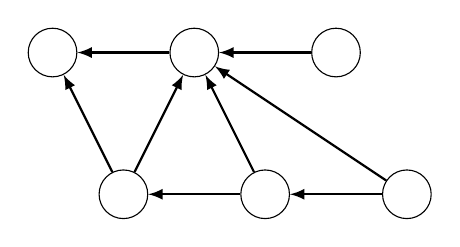
\begin{tikzpicture}[scale=0.9]
\node[draw, circle] (1) at (0,0) {\phantom{0}};
\node[draw, circle] (2) at (2,0) {\phantom{0}};
\node[draw, circle] (3) at (4,0) {\phantom{0}};
\node[draw, circle] (4) at (1,-2) {\phantom{0}};
\node[draw, circle] (5) at (3,-2) {\phantom{0}};
\node[draw, circle] (6) at (5,-2) {\phantom{0}};

\path[draw,thick,->,>=latex] (2) -- (1);
\path[draw,thick,->,>=latex] (3) -- (2);
\path[draw,thick,->,>=latex] (5) -- (4);
\path[draw,thick,->,>=latex] (6) -- (5);
\path[draw,thick,->,>=latex] (4) -- (1);
\path[draw,thick,->,>=latex] (4) -- (2);
\path[draw,thick,->,>=latex] (5) -- (2);
\path[draw,thick,->,>=latex] (6) -- (2);
\end{tikzpicture}
\end{center}
Гранди сандары келесідей:
\begin{center}
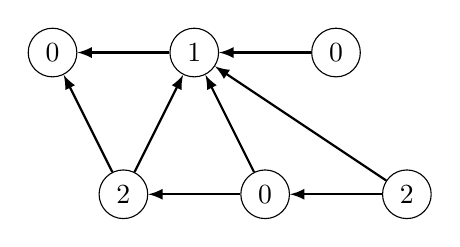
\begin{tikzpicture}[scale=0.9]
\node[draw, circle] (1) at (0,0) {0};
\node[draw, circle] (2) at (2,0) {1};
\node[draw, circle] (3) at (4,0) {0};
\node[draw, circle] (4) at (1,-2) {2};
\node[draw, circle] (5) at (3,-2) {0};
\node[draw, circle] (6) at (5,-2) {2};

\path[draw,thick,->,>=latex] (2) -- (1);
\path[draw,thick,->,>=latex] (3) -- (2);
\path[draw,thick,->,>=latex] (5) -- (4);
\path[draw,thick,->,>=latex] (6) -- (5);
\path[draw,thick,->,>=latex] (4) -- (1);
\path[draw,thick,->,>=latex] (4) -- (2);
\path[draw,thick,->,>=latex] (5) -- (2);
\path[draw,thick,->,>=latex] (6) -- (2);
\end{tikzpicture}
\end{center}
Ұтылыс күйінің Гранди саны -- 0, ал ұтыс күйінің
Гранди саны -- оң сан.
% The Grundy number of a losing state is 0,
% and the Grundy number of a winning state is
% a positive number.

Күйдегі Гранди саны ним үйіндісіндегі таяқтар санына
сәйкес келеді. Егер Гранди саны 0 болса, біз тек
Гранди саны оң болатын күйлерге бара аламыз. Ал егер 
Гранди саны $x>0$ болса, онда біз 
Гранди саны $0,1,\ldots,x-1$ болатын барлық
күйлерге бара аламыз. 

% The Grundy number of a state corresponds to
% the number of sticks in a nim heap.
% If the Grundy number is 0, we can only move to
% states whose Grundy numbers are positive,
% and if the Grundy number is $x>0$, we can move
% to states whose Grundy numbers include all numbers
% $0,1,\ldots,x-1$.

Мысал ретінде ойыншылар лабиринттегі фигураны 
жылжытатын ойынды қарастырайық. Лабиринттегі 
әр шаршы не еденді, не қабырғаны білдіреді. 
Әр жүріс сайын ойыншы фигураны бірнеше қадам солға немесе үстіге 
жылжытуы керек. Соңғы жүрісті жасаған ойыншы жеңіске жетеді. 

% As an example, consider a game where
% the players move a figure in a maze.
% Each square in the maze is either floor or wall.
% On each turn, the player has to move
% the figure some number
% of steps left or up.
% The winner of the game is the player who
% makes the last move.

Келесі сурет ойынның күйін көрсетеді, мұнда @
таңбасы фигураның орналасуын белгілейді және * таңбасы
жүріс жасай алатын торларды белгілейді. 

% The following picture shows a possible initial state
% of the game, where @ denotes the figure and *
% denotes a square where it can move.

\begin{center}
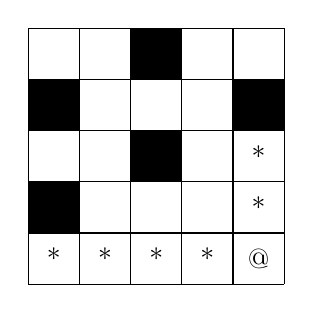
\begin{tikzpicture}[scale=.65]
  \begin{scope}
    \fill [color=black] (0, 1) rectangle (1, 2);
    \fill [color=black] (0, 3) rectangle (1, 4);
    \fill [color=black] (2, 2) rectangle (3, 3);
    \fill [color=black] (2, 4) rectangle (3, 5);
    \fill [color=black] (4, 3) rectangle (5, 4);

    \draw (0, 0) grid (5, 5);
    
    \node at (4.5,0.5) {@};
    \node at (3.5,0.5) {*};
    \node at (2.5,0.5) {*};
    \node at (1.5,0.5) {*};
    \node at (0.5,0.5) {*};
    \node at (4.5,1.5) {*};
    \node at (4.5,2.5) {*};
    
  \end{scope}
\end{tikzpicture}
\end{center}

Ойынның күйлері -- лабиринт еденіндегі барлық шаршылар. 
Жоғарыда келтірілген лабиринттегі Гранди сандары келесідей:
% The states of the game are all floor squares
% of the maze.
% In the above maze, the Grundy numbers
% are as follows:

\begin{center}
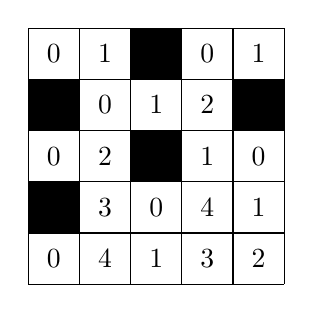
\begin{tikzpicture}[scale=.65]
  \begin{scope}
    \fill [color=black] (0, 1) rectangle (1, 2);
    \fill [color=black] (0, 3) rectangle (1, 4);
    \fill [color=black] (2, 2) rectangle (3, 3);
    \fill [color=black] (2, 4) rectangle (3, 5);
    \fill [color=black] (4, 3) rectangle (5, 4);

    \draw (0, 0) grid (5, 5);
    
    \node at (0.5,4.5) {0};
    \node at (1.5,4.5) {1};
    \node at (2.5,4.5) {};
    \node at (3.5,4.5) {0};
    \node at (4.5,4.5) {1};

    \node at (0.5,3.5) {};
    \node at (1.5,3.5) {0};
    \node at (2.5,3.5) {1};
    \node at (3.5,3.5) {2};
    \node at (4.5,3.5) {};

    \node at (0.5,2.5) {0};
    \node at (1.5,2.5) {2};
    \node at (2.5,2.5) {};
    \node at (3.5,2.5) {1};
    \node at (4.5,2.5) {0};

    \node at (0.5,1.5) {};
    \node at (1.5,1.5) {3};
    \node at (2.5,1.5) {0};
    \node at (3.5,1.5) {4};
    \node at (4.5,1.5) {1};

    \node at (0.5,0.5) {0};
    \node at (1.5,0.5) {4};
    \node at (2.5,0.5) {1};
    \node at (3.5,0.5) {3};
    \node at (4.5,0.5) {2};
  \end{scope}
\end{tikzpicture}
\end{center}

Лабиринттегі әр күй ним ойындағы үйіндіге сәйкес келеді.
Мысалы, төменгі оң жақтағы шаршының Гранди саны 2,
демек бұл -- ұтыс күйі. Ал фигураны 4 қадам солға немесе 2 қадам үстіге жылжытсақ, ұтылыс күйіне жетеміз. 

% Thus, each state of the maze game
% corresponds to a heap in the nim game.
% For example, the Grundy number for
% the lower-right square is 2,
% so it is a winning state.
% We can reach a losing state and
% win the game by moving
% either four steps left or
% two steps up.

Ним ойынына қарағанда 
қазіргі күйдің Гранди санынан үлкен 
күйге өтуге болатынын ескергеніміз жөн. % TODO
Бірақ қарсылас сондай жүрістің күшін жоятын 
жүрісті әрдайым таңдай алады. Демек ұтылыс 
күйінен қашу мүмкін емес. 


% Note that unlike in the original nim game,
% it may be possible to move to a state whose
% Grundy number is larger than the Grundy number
% of the current state.
% However, the opponent can always choose a move
% that cancels such a move, so it is not possible
% to escape from a losing state.

\subsubsection{Ішойындар}

Ойын ішойындардан тұрады делік. Әр жүрісте
ойыншы бірінші ішойынды, содан кейін сол ішойындағы жүрісті таңдайды. 
Ойыншылардың ешқайсысы ешбір ішойында жүріс жасай алмайтындай болған кезде ойын аяқталады.

% Next we will assume that our game consists
% of subgames, and on each turn, the player
% first chooses a subgame and then a move in the subgame.
% The game ends when it is not possible to make any move
% in any subgame.

Бұл жағдайда ойынның Гранди саны ішойындардың
Гранди сандарының ним қосындысына тең болады. Ойынды ішойындардың барлық Гранди сандарын, содан кейін олардың ним қосындысын есептеу арқылы қарапайым
ним ойыны сияқты ойнауға болады. 

% In this case, the Grundy number of a game
% is the nim sum of the Grundy numbers of the subgames.
% The game can be played like a nim game by calculating
% all Grundy numbers for subgames and then their nim sum.

Мысалы 3 лабиринттен тұратын ойынды қарастырайық. 
Бұл ойында әр жүрісте ойыншы бір лабиринтті таңдап,
соның ішіндегі фигураны жылжытады. Ойынның бастапқы күйі
келесідей делік:

% As an example, consider a game that consists
% of three mazes.
% In this game, on each turn, the player chooses one
% of the mazes and then moves the figure in the maze.
% Assume that the initial state of the game is as follows:

\begin{center}
\begin{tabular}{ccc}
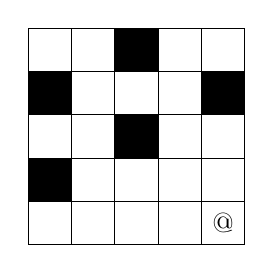
\begin{tikzpicture}[scale=.55]
  \begin{scope}
    \fill [color=black] (0, 1) rectangle (1, 2);
    \fill [color=black] (0, 3) rectangle (1, 4);
    \fill [color=black] (2, 2) rectangle (3, 3);
    \fill [color=black] (2, 4) rectangle (3, 5);
    \fill [color=black] (4, 3) rectangle (5, 4);

    \draw (0, 0) grid (5, 5);

    \node at (4.5,0.5) {@};

    \end{scope}
\end{tikzpicture}
&
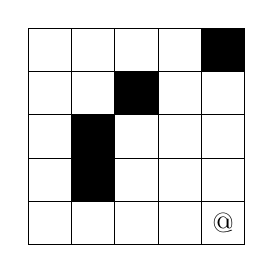
\begin{tikzpicture}[scale=.55]
  \begin{scope}
    \fill [color=black] (1, 1) rectangle (2, 3);
    \fill [color=black] (2, 3) rectangle (3, 4);
    \fill [color=black] (4, 4) rectangle (5, 5);

    \draw (0, 0) grid (5, 5);
    
    \node at (4.5,0.5) {@};

  \end{scope}
\end{tikzpicture}
&
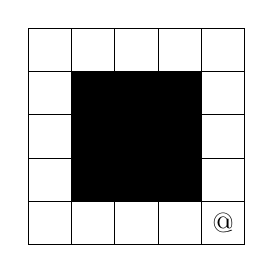
\begin{tikzpicture}[scale=.55]
  \begin{scope}
    \fill [color=black] (1, 1) rectangle (4, 4);

    \draw (0, 0) grid (5, 5);
    
    \node at (4.5,0.5) {@};
  \end{scope}
\end{tikzpicture}
\end{tabular}
\end{center}

Лабиринттердің Гранди сандары келесідей:

\begin{center}
\begin{tabular}{ccc}
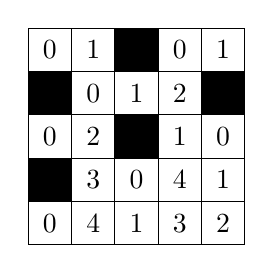
\begin{tikzpicture}[scale=.55]
  \begin{scope}
    \fill [color=black] (0, 1) rectangle (1, 2);
    \fill [color=black] (0, 3) rectangle (1, 4);
    \fill [color=black] (2, 2) rectangle (3, 3);
    \fill [color=black] (2, 4) rectangle (3, 5);
    \fill [color=black] (4, 3) rectangle (5, 4);

    \draw (0, 0) grid (5, 5);

    \node at (0.5,4.5) {0};
    \node at (1.5,4.5) {1};
    \node at (2.5,4.5) {};
    \node at (3.5,4.5) {0};
    \node at (4.5,4.5) {1};

    \node at (0.5,3.5) {};
    \node at (1.5,3.5) {0};
    \node at (2.5,3.5) {1};
    \node at (3.5,3.5) {2};
    \node at (4.5,3.5) {};

    \node at (0.5,2.5) {0};
    \node at (1.5,2.5) {2};
    \node at (2.5,2.5) {};
    \node at (3.5,2.5) {1};
    \node at (4.5,2.5) {0};

    \node at (0.5,1.5) {};
    \node at (1.5,1.5) {3};
    \node at (2.5,1.5) {0};
    \node at (3.5,1.5) {4};
    \node at (4.5,1.5) {1};

    \node at (0.5,0.5) {0};
    \node at (1.5,0.5) {4};
    \node at (2.5,0.5) {1};
    \node at (3.5,0.5) {3};
    \node at (4.5,0.5) {2};
    \end{scope}
\end{tikzpicture}
&
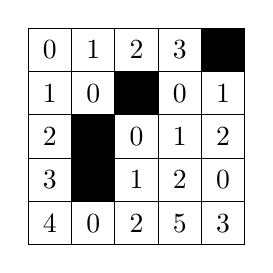
\begin{tikzpicture}[scale=.55]
  \begin{scope}
    \fill [color=black] (1, 1) rectangle (2, 3);
    \fill [color=black] (2, 3) rectangle (3, 4);
    \fill [color=black] (4, 4) rectangle (5, 5);

    \draw (0, 0) grid (5, 5);

    \node at (0.5,4.5) {0};
    \node at (1.5,4.5) {1};
    \node at (2.5,4.5) {2};
    \node at (3.5,4.5) {3};
    \node at (4.5,4.5) {};

    \node at (0.5,3.5) {1};
    \node at (1.5,3.5) {0};
    \node at (2.5,3.5) {};
    \node at (3.5,3.5) {0};
    \node at (4.5,3.5) {1};

    \node at (0.5,2.5) {2};
    \node at (1.5,2.5) {};
    \node at (2.5,2.5) {0};
    \node at (3.5,2.5) {1};
    \node at (4.5,2.5) {2};

    \node at (0.5,1.5) {3};
    \node at (1.5,1.5) {};
    \node at (2.5,1.5) {1};
    \node at (3.5,1.5) {2};
    \node at (4.5,1.5) {0};

    \node at (0.5,0.5) {4};
    \node at (1.5,0.5) {0};
    \node at (2.5,0.5) {2};
    \node at (3.5,0.5) {5};
    \node at (4.5,0.5) {3};
  \end{scope}
\end{tikzpicture}
&
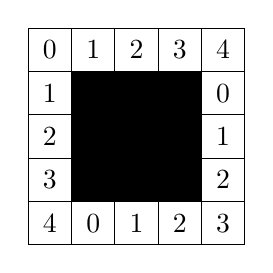
\begin{tikzpicture}[scale=.55]
  \begin{scope}
    \fill [color=black] (1, 1) rectangle (4, 4);

    \draw (0, 0) grid (5, 5);

    \node at (0.5,4.5) {0};
    \node at (1.5,4.5) {1};
    \node at (2.5,4.5) {2};
    \node at (3.5,4.5) {3};
    \node at (4.5,4.5) {4};

    \node at (0.5,3.5) {1};
    \node at (1.5,3.5) {};
    \node at (2.5,3.5) {};
    \node at (3.5,3.5) {};
    \node at (4.5,3.5) {0};

    \node at (0.5,2.5) {2};
    \node at (1.5,2.5) {};
    \node at (2.5,2.5) {};
    \node at (3.5,2.5) {};
    \node at (4.5,2.5) {1};

    \node at (0.5,1.5) {3};
    \node at (1.5,1.5) {};
    \node at (2.5,1.5) {};
    \node at (3.5,1.5) {};
    \node at (4.5,1.5) {2};

    \node at (0.5,0.5) {4};
    \node at (1.5,0.5) {0};
    \node at (2.5,0.5) {1};
    \node at (3.5,0.5) {2};
    \node at (4.5,0.5) {3};
  \end{scope}
\end{tikzpicture}
\end{tabular}
\end{center}

Әуелгі күйде Гранди сандарының ним қосындысы $2 \oplus 3 \oplus 3 = 2$,
демек бірінші ойыншы жеңеді. Тиімді жүрістердің бірі -- 
бірінші лабиринтте 2 қадам фигураны алдығы жылжыту. Ол
$0 \oplus 3 \oplus 3 = 0$ ним қосындысын береді. 

% In the initial state, the nim sum of the Grundy numbers
% is $2 \oplus 3 \oplus 3 = 2$, so
% the first player can win the game.
% One optimal move is to move two steps up
% in the first maze, which produces the nim sum
% $0 \oplus 3 \oplus 3 = 0$.

\subsubsection{Гранди ойыны}

Кейде ойындағы жүріс ойынды өзара тәуелсіз 
бірнеше ішойындарға бөледі. Ондай кездегі 
ойынның Гранди саны 

% Sometimes a move in a game divides the game
% into subgames that are independent of each other.
% In this case, the Grundy number of the game is

\[\textrm{mex}(\{g_1, g_2, \ldots, g_n \}),\]
мұндағы $n$ мүмкін болатын жүрістер саны және
% where $n$ is the number of possible moves and
\[g_k = a_{k,1} \oplus a_{k,2} \oplus \ldots \oplus a_{k,m},\]
мұндағы $k$ жүрісі Гранди сандары $a_{k,1},a_{k,2},\ldots,a_{k,m}$ болатын
ішойындарды өндіреді. 
% where move $k$ generates subgames with
% Grundy numbers $a_{k,1},a_{k,2},\ldots,a_{k,m}$.

\index{Гранди ойыны}

Сондай ойындардың мысалы ретінде \key{Гранди ойынын} келтіруімізге болады. 
Басында бізге $n$ таяқтан тұратын бір үйінді берілген делік.
Әр жүрісте ойыншы үйіндіні таңдап, бос емес және өлшемдері
әртүрлі екі үйіндіге бөледі. Соңғы болып жүрген 
ойыншы жеңеді. 

% An example of such a game is \key{Grundy's game}.
% Initially, there is a single heap that contains $n$ sticks.
% On each turn, the player chooses a heap and divides
% it into two nonempty heaps such that the heaps
% are of different size.
% The player who makes the last move wins the game.

$f(n)$ деп $n$ таяқтан тұратын үйіндідегі Гранди санын белгілейік. Гранди санын үйіндіні екі үйіндіге бөлудің барлық жолдарын қолдану арқылы есептеуімізге болады. Мысалы $n=8$ болған кезде,
бөлу мүмкіндіктері $1+7$, $2+6$ және $3+5$ болады.
Демек \[f(8)=\textrm{mex}(\{f(1) \oplus f(7), f(2) \oplus f(6), f(3) \oplus f(5)\}).\]


% Let $f(n)$ be the Grundy number of a heap
% that contains $n$ sticks.
% The Grundy number can be calculated by going
% through all ways to divide the heap into
% two heaps.
% For example, when $n=8$, the possibilities
% are $1+7$, $2+6$ and $3+5$, so
% \[f(8)=\textrm{mex}(\{f(1) \oplus f(7), f(2) \oplus f(6), f(3) \oplus f(5)\}).\]

Осы ойында $f(n)$ мәні $f(1),\ldots,f(n-1)$ мәндеріне
негізделеді. Функцияның негізгі жағдайлары $f(1)=f(2)=0$,
себебі 1 және 2 таяқтан тұратын үйінділерді бөлу мүмкін емес. 
Алғашқы Гранди сандары:

% In this game, the value of $f(n)$ is based on the values
% of $f(1),\ldots,f(n-1)$.
% The base cases are $f(1)=f(2)=0$,
% because it is not possible to divide the heaps
% of 1 and 2 sticks.
% The first Grundy numbers are:
\[
\begin{array}{lcl}
f(1) & = & 0 \\
f(2) & = & 0 \\
f(3) & = & 1 \\
f(4) & = & 0 \\
f(5) & = & 2 \\
f(6) & = & 1 \\
f(7) & = & 0 \\
f(8) & = & 2 \\
\end{array}
\]
Гранди саны $n=8$ үшін 2-ге тең, демек ойынды ұтуға болады. 
Ұтыс жүріске $1+7$ үйінділерін құру арқылы қол жеткіземіз.
Себебі $f(1) \oplus f(7) = 0$ болады.
% The Grundy number for $n=8$ is 2,
% so it is possible to win the game.
% The winning move is to create heaps
% $1+7$, because $f(1) \oplus f(7) = 0$.

